	Sea la transformación $R$:
	\[
	R(\theta) = \begin{bmatrix} \cos \theta & -\sin \theta \\[3pt] \sin \theta & \cos \theta \\ \end{bmatrix}
	\]

\begin{enumerate}
	\item Genere y grafique un Vector en $\Re^2$

		\textbf{R:}\\

		Generamos el vector usando la función rand() en cada componente del mismo (en octave).
		Luego, graficamos el vector generado usando plot:

		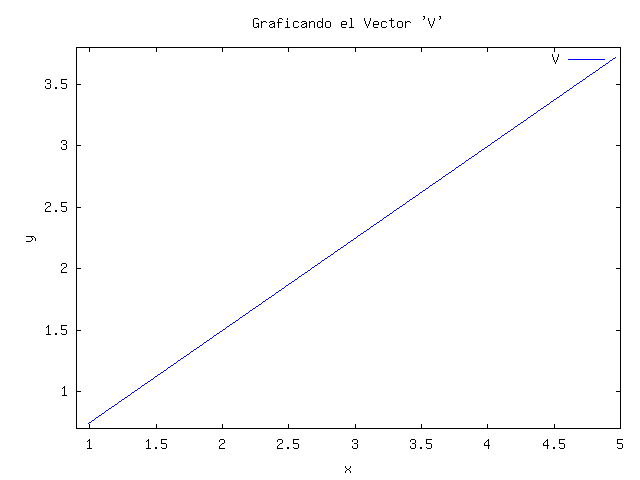
\includegraphics[scale=0.6]{imagenes/3_v.png}
	\newpage
	\item Al vector generado, aplique la transformación propuesta con argumento $17$, $31$, $47$,
		$61$, $97$, ¿Qué efecto puede ver?

		\textbf{R:}\\
	
		Analizando los gráficos:\\
		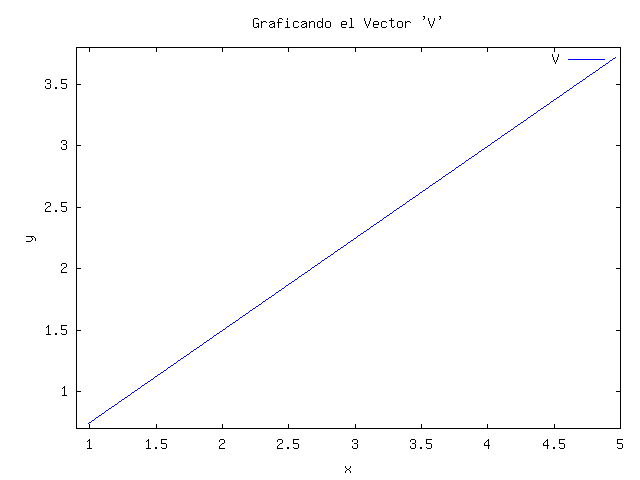
\includegraphics[scale=0.3]{imagenes/3_v.png}
		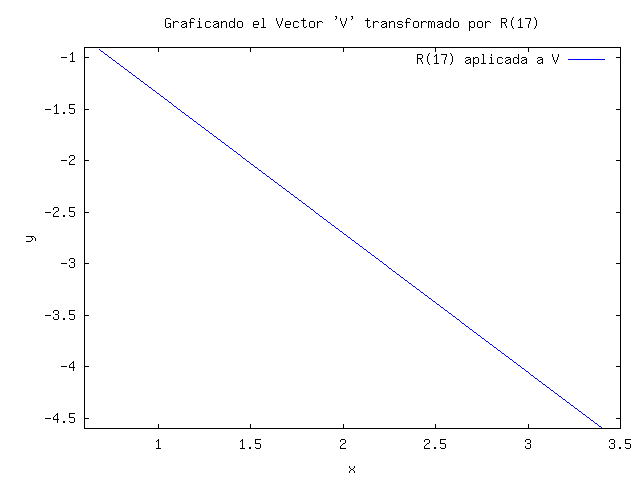
\includegraphics[scale=0.3]{imagenes/3_va.png}\\
		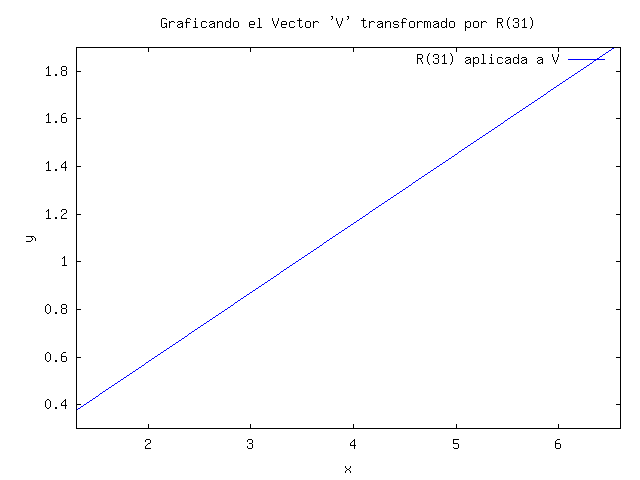
\includegraphics[scale=0.3]{imagenes/3_vb.png}
		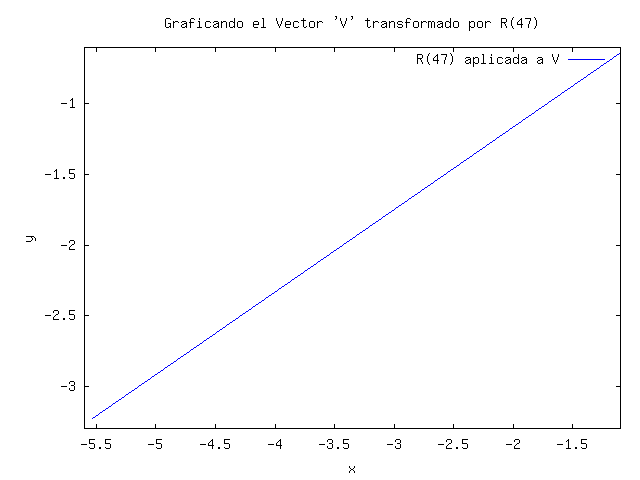
\includegraphics[scale=0.3]{imagenes/3_vc.png}\\
		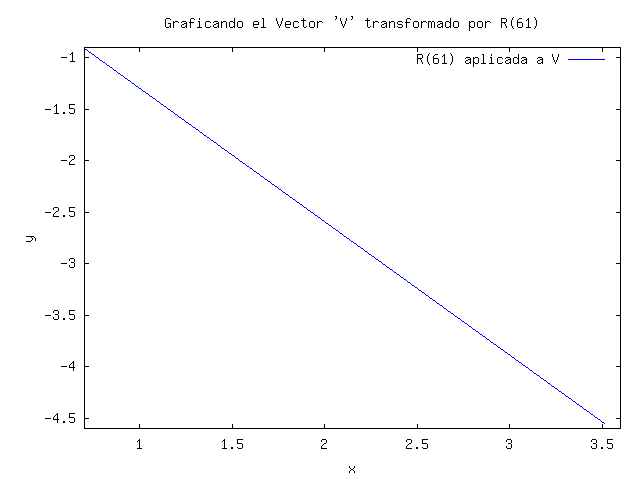
\includegraphics[scale=0.3]{imagenes/3_vd.png}
		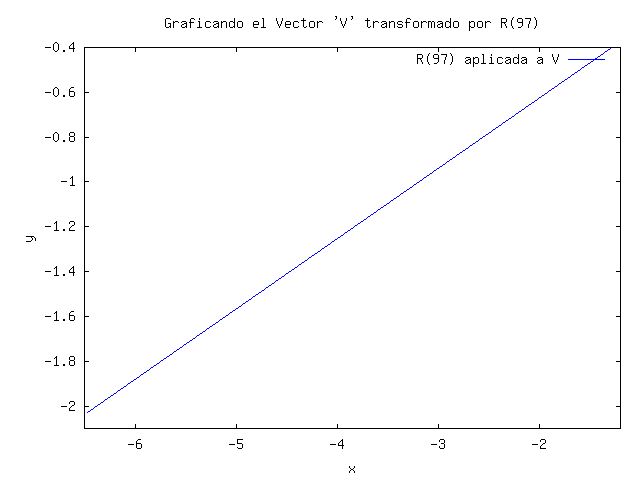
\includegraphics[scale=0.3]{imagenes/3_ve.png}
		
		Nos podemos dar cuenta que las transformaciones sólo rotan al vector sobre el eje de
		coordenadas.
		\newpage
	\item Realice el mismo ejercicio para un vector en $\Re^3$

		\textbf{R:}\\

		De la misma forma, generamos y graficamos un vector (ahora usando plot3):\\
		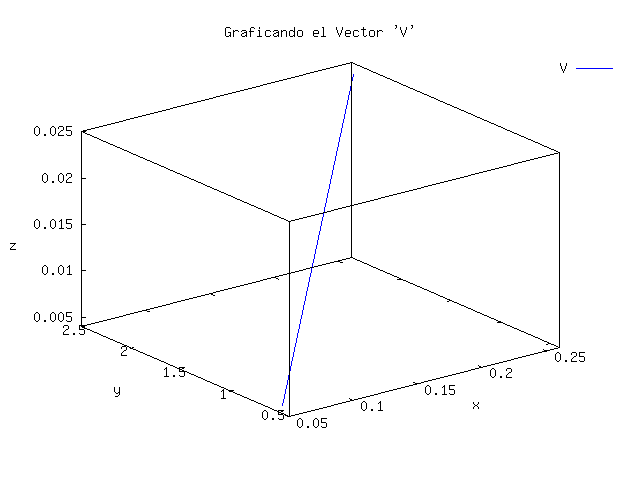
\includegraphics[scale=0.6]{imagenes/3_v3.png}

		Ahora, simplemente en vez de usar la matriz de transformación de $\Re^2$, la pasamos a
		$\Re^3$ dejando que al ser aplicada rote sobre el eje x:
		\[
		R_x(\theta) = \begin{bmatrix} 1 & 0 & 0 \\ 0 & \cos \theta	& -\sin \theta \\[3pt] 0 & \sin \theta  & \cos \theta \\[3pt] \end{bmatrix}\\[6pt] 
		\]

		\newpage
		Y revisando los gráficos:\\
		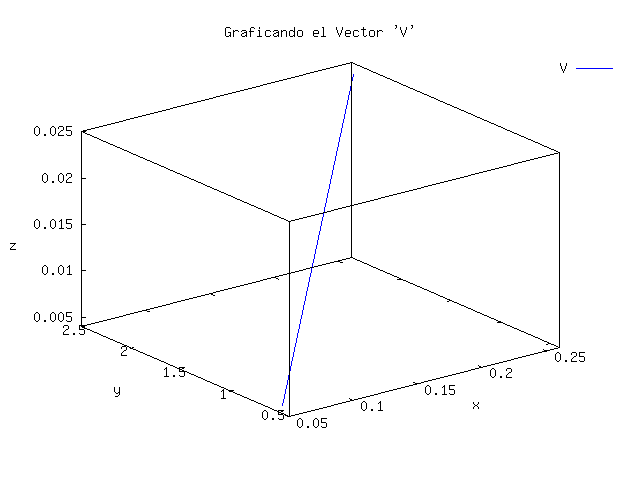
\includegraphics[scale=0.3]{imagenes/3_v3.png}
		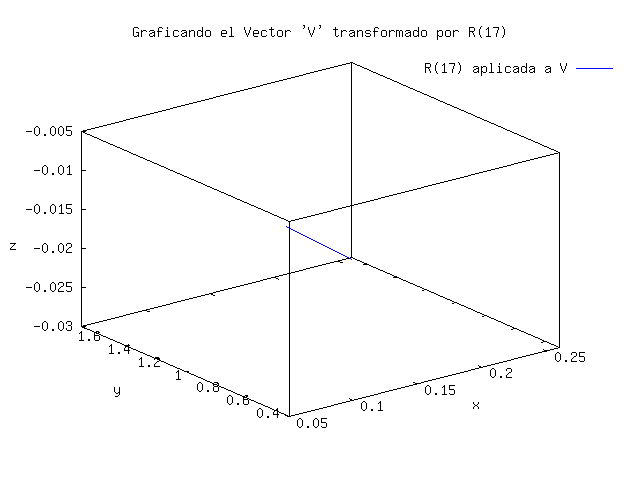
\includegraphics[scale=0.3]{imagenes/3_va3.png}\\
		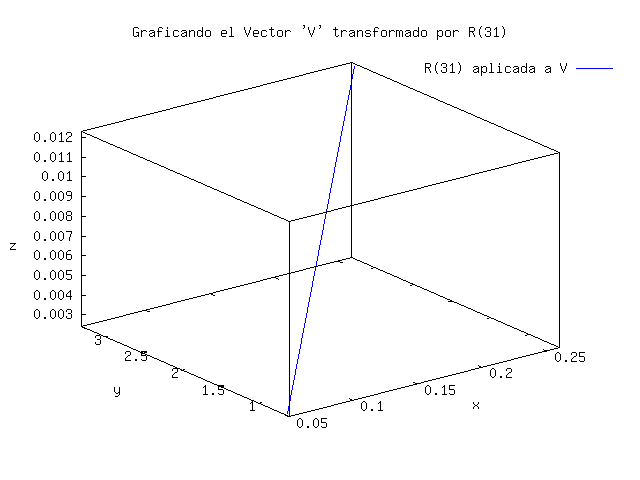
\includegraphics[scale=0.3]{imagenes/3_vb3.png}
		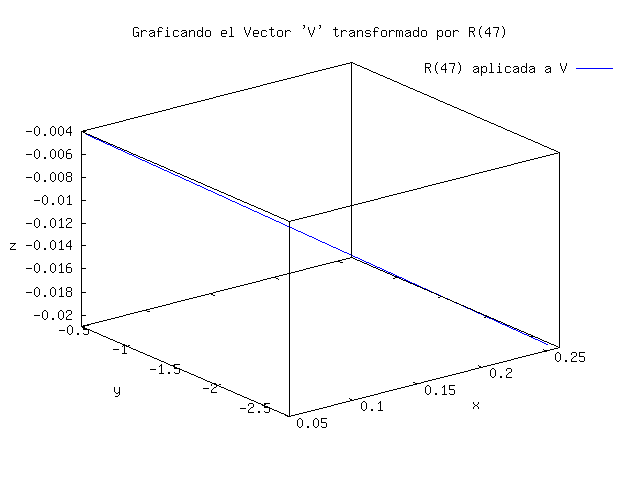
\includegraphics[scale=0.3]{imagenes/3_vc3.png}\\
		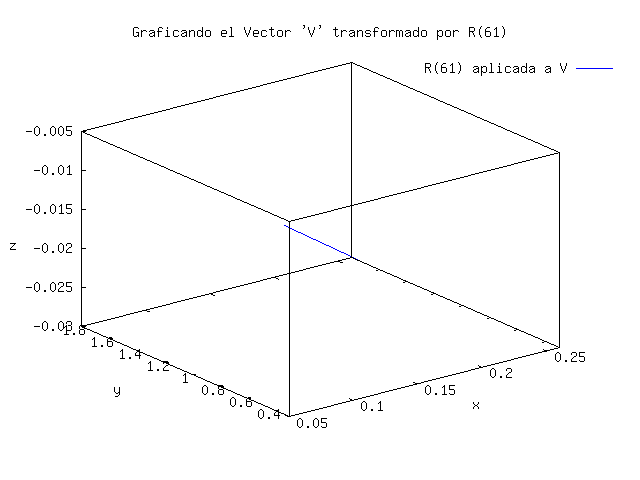
\includegraphics[scale=0.3]{imagenes/3_vd3.png}
		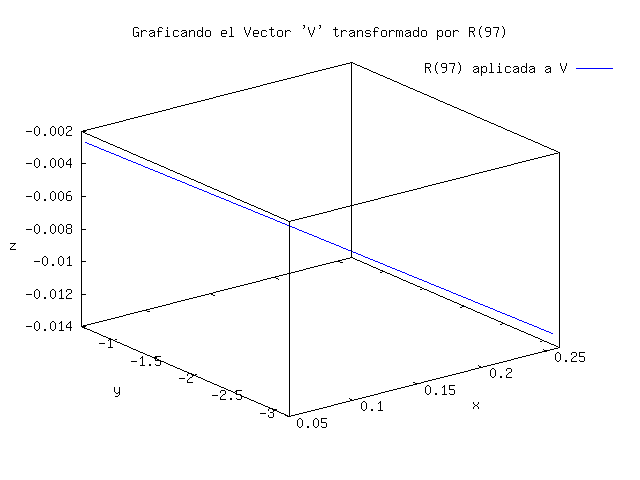
\includegraphics[scale=0.3]{imagenes/3_ve3.png}

		Podemos concluir que la transformación $R_x(\theta)$ en $\Re^3$, al igual que la transformación $R$
		en $\Re^2$, rota el vector en torno a los ejes de coordenadas.
\end{enumerate}
